\documentclass{article}

\usepackage{times}
\usepackage{geometry}
\geometry{a4paper,left=0.6cm,right=0.7cm,top=2cm,bottom=1cm,columnsep=0.8cm}
\usepackage{fontawesome}
\usepackage[hidelinks]{hyperref}
\usepackage{multicol}
\usepackage{tikz}
\usepackage{hyphsubst}
\usepackage{moresize}
\usepackage{hyphenat}
\usepackage{tabularx}
\usepackage{xcolor}
\usepackage{enumitem}
\usetikzlibrary{calc, positioning}      
\newcolumntype{Y}{>{\RaggedRight\arraybackslash}X}

% Définition des couleurs
\definecolor{maincolor}{HTML}{f0fafc}
\definecolor{seccolor}{HTML}{ffffff}
\definecolor{gray}{HTML}{8c94a9}
\definecolor{sidetext}{HTML}{59cee5}

% Solution robuste pour la bande bleue sur toute la hauteur
\usepackage{eso-pic}
\AddToShipoutPictureBG{%
  \begin{tikzpicture}[remember picture,overlay]
    \fill[maincolor] 
        (current page.north west) rectangle 
        ([xshift=0.3\paperwidth] current page.south west);
  \end{tikzpicture}%
}

% Configuration des listes
\setlist[itemize]{itemsep=-2pt,topsep=0pt,leftmargin=1.08cm}
\renewcommand{\labelitemi}{\textcolor{sidetext}{\footnotesize$\bullet$}}

\setlength{\parindent}{0pt}
\usepackage{paracol}
\columnratio{0.3}

\begin{document}

\pagestyle{empty}

\begin{paracol}{2}
% -----------------------------------------------------------------
% Colonne gauche
% -----------------------------------------------------------------
\color{sidetext}
\begin{center}
    \begin{tikzpicture}
        \clip (0,0) circle (1.5cm) node[anchor=center] {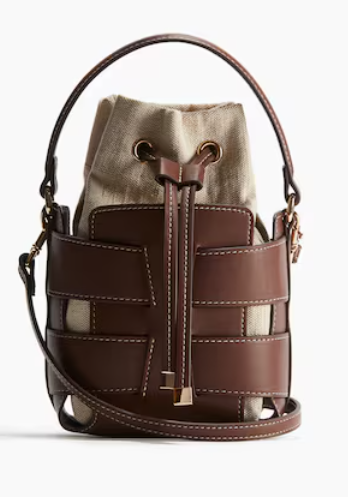
\includegraphics[width=3cm]{a971b307ea334c1abf7fcc2448e8274e.png}};
    \end{tikzpicture}

    \vspace{5mm}
    
    {\color{black}\LARGE \textbf{Dora SARKIS}}
    
    \vspace{3mm}
    
    {\large{Gérante \& Directrice}}
\end{center}

{\color{gray}\rule{\linewidth}{0.4pt}} \\

% Coordonnées
\begin{tabular}{@{}c l}
    \faPhone{} & 
    \begin{tabular}[t]{@{}l@{}}
        {\color{gray}Téléphone} \\
        06\,90\,59\,69\,69
    \end{tabular} \\
    \\
    \faEnvelope{} & 
    \begin{tabular}[t]{@{}l@{}}
        {\color{gray}Mail} \\
        leroyalriviera@gmail.com
    \end{tabular} \\
    \\
    \faMapMarker{} & 
    \begin{tabular}[t]{@{}l@{}}
        {\color{gray}Adresse} \\
        53 résidence Les Citronnelles
    \end{tabular} \\
\end{tabular}

\vspace{5mm}
{\color{gray}\rule{\linewidth}{0.4pt}} \\

% Compétences
{\color{black}{Compétences Clés}}

\vspace{4mm}

\begin{tabular}{@{}c l}
    \textcolor{sidetext}{\faUsers} & Gestion d’entreprise \\
    \\
    \textcolor{sidetext}{\faHandshakeO} & Négociation commerciale \\
    \\
    \textcolor{sidetext}{\faAddressBookO} & Relation client \\
    \\
    \textcolor{sidetext}{\faCalendarCheckO} & Organisation d’événements \\
    \\
    \textcolor{sidetext}{\faLineChart} & Management \& gestion administrative \\
    \\
    \textcolor{sidetext}{\faGavel} & Sens de l’organisation, autonomie \\
\end{tabular}

% Espace flexible pour étendre la colonne gauche
\vfill
~

\switchcolumn
% -----------------------------------------------------------------
% Colonne droite
% -----------------------------------------------------------------
\color{black}

% Profil
\textcolor{black}{\Large \textbf{Profil Professionnel}} \\[2pt]

Gérante et directrice polyvalente disposant de plus de 10 ans d’expérience dans la création, la gestion et le développement de structures commerciales et culturelles. Spécialisée dans la négociation, la relation client et l’organisation d’événements à forte valeur ajoutée. Habituée à piloter des équipes pluridisciplinaires et à assurer le suivi administratif et financier d’activités variées. Passionnée par le droit commercial et immobilier, elle conjugue rigueur, autonomie et sens aigu de l’organisation pour faire croître les projets qui lui sont confiés. \\[8pt]

% Expérience
\textcolor{black}{\Large \textbf{Expérience Professionnelle}} \\

% Expérience 1
\colorbox{maincolor}{%
  \begin{minipage}{\linewidth}
    \begin{tabular}{@{}l l r}
        \textcolor{sidetext}{\faBriefcase} & 
        \textbf{Gérante – Boutique \& Locaux commerciaux} &  
        \footnotesize{2019 -- Présent} \\
        & \textit{Pointe-à-Pitre} & \\
    \end{tabular}
    \begin{itemize}
        \item Supervision d’une boutique de détail et gestion locative de plusieurs espaces commerciaux. 
        \item Négociation avec fournisseurs et locataires, suivi administratif et comptable complet. 
        \item Mise en place d’actions commerciales visant à accroître la fréquentation et le chiffre d’affaires.
    \end{itemize}
  \end{minipage}%
}

\vspace{5mm}

% Expérience 2
\colorbox{maincolor}{%
  \begin{minipage}{\linewidth}
    \begin{tabular}{@{}l l r}
        \textcolor{sidetext}{\faBriefcase} & 
        \textbf{Directrice – Salle de spectacle} &  
        \footnotesize{2012 -- 2018} \\
    \end{tabular}
    \begin{itemize}
        \item Pilotage de la programmation et de l’organisation logistique d’événements culturels variés. 
        \item Management opérationnel des équipes et gestion budgétaire de la structure. 
        \item Développement de partenariats afin d’optimiser la fréquentation et la rentabilité.
    \end{itemize}
  \end{minipage}%
}

\vspace{5mm}

% Expérience 3
\colorbox{maincolor}{%
  \begin{minipage}{\linewidth}
    \begin{tabular}{@{}l l r}
        \textcolor{sidetext}{\faBriefcase} & 
        \textbf{Gérante fondatrice – Joykiss} &  
        \footnotesize{2008 -- 2012} \\
    \end{tabular}
    \begin{itemize}
        \item Création et gestion d’une boutique spécialisée dans le mariage, incluant services de wedding planning et design. 
        \item Négociation avec prestataires, accompagnement personnalisé des clients et développement de nouvelles offres. 
        \item Mise en place de processus internes assurant qualité de service et rentabilité.
    \end{itemize}
  \end{minipage}%
}

\vspace{8mm}

% Formation
\textcolor{black}{\Large \textbf{Formation}} \\[4pt]

\begin{tabular}{@{}c l}
    \textcolor{sidetext}{\faGraduationCap} & 
    \begin{tabular}[t]{@{}l@{}}
        \textbf{Formation en décoration événementielle} \\
        Centre ABC, 2008 \\
        Approfondissement des techniques de design et scénographie pour événements.
    \end{tabular} \\
\end{tabular}

\vspace{4mm}

\begin{tabular}{@{}c l}
    \textcolor{sidetext}{\faGraduationCap} & 
    \begin{tabular}[t]{@{}l@{}}
        \textbf{BTS Commerce international (inachevé)} \\
        CNED, 2008 \\
        Enseignements orientés négociation, import-export et pratiques commerciales internationales.
    \end{tabular} \\
\end{tabular}

\vspace{4mm}

\begin{tabular}{@{}c l}
    \textcolor{sidetext}{\faGraduationCap} & 
    \begin{tabular}[t]{@{}l@{}}
        \textbf{Baccalauréat professionnel Commerce} \\
        CNED, 2006 \\
        Formation axée sur la vente, la gestion de la relation client et le marketing opérationnel.
    \end{tabular} \\
\end{tabular}

\vspace{8mm}
\end{paracol}

\end{document}